\documentclass[MAIN.tex]{subfiles}

% Load any packages needed for this document
\begin{document}
	
		\section{Regression Methods}
	Conventional regression models are estimated using the ordinary
	least squares (OLS) technique, and are referred to as `Model I
	regression'\citep{CornCoch,ludbrook97}. A key feature of Model I
	models is that the independent variable is assumed to be measured
	without error. As often pointed out in several papers
	\citep{BA83,ludbrook97}, this assumption invalidates simple linear
	regression for use in method comparison studies, as both methods
	must be assumed to be measured with error.
	
	The use of regression models that assumes the presence of error in
	both variables $X$ and $Y$ have been proposed for use instead.
	\citep{CornCoch,ludbrook97}, These methodologies are collectively
	known as `Model II regression'. They differ in the method used to
	estimate the parameters of the regression.
	
	Regression estimates depend on formulation of the model. A formulation with one method considered as the $X$ variable will 	yield different estimates for a formulation where it is the $Y$ variable. With Model I regression,the models fitted in both cases
	will entirely different and inconsistent. However with Model II	regression, they will be consistent and complementary.

	
Regression approaches are useful for a making a detailed examination of the biases across the range of measurements, allowing bias to be decomposed into fixed bias and proportional bias. Fixed bias describes the case where one method gives values that are consistently different	to the other across the whole range. Proportional bias describes the difference in measurements getting progressively greater, or smaller, across the range of measurements. A measurement method may have either an attendant fixed bias or proportional bias, or both. \citep{ludbrook}. Determination of these biases shall be discussed in due course.

\subsection{Simple Linear Regression} Simple Linear Regression is  well
known statistical technique , wherein estimates for slope and intercept of the line of best fit are derived according to the
Ordinary Least Square (OLS) principle.This method is known to Cornbleet and Cochrane as Model I regression.
\\
\\
In Model I regression, the independent variable is assumed to be
measured without error. For method comparison studies, both sets of measurement must be assumed to be measured with imprecision and
neither case can be taken to be a reference method. Arbitrarily selecting either method as the reference will yield two
conflicting outcomes. A fitting based on '$X$ on $Y$' will give inconsistent results with a fitting based on '$Y$ on $X$'.
Consequently model I regression is inappropriate for such cases.
\\
\\
Conversely, Cornbleet Cochrane state that when the independent variable $X$ is a precisely measured reference method, Model I
regression may be considered suitable. They qualify this statement
by referring the $X$ as \emph{the 'correct' value}, tacitly implying that there must still be some measurement error present.
The validity of this approach has been disputed elsewhere.

\section{Model II Regression}

\subsection{Model II regression}
Cochrane and Cornbleet argue for the use of methods that based on
the assumption that both methods are imprecisely measured ,and
that yield a fitting that is consistent with both '$X$ on $Y$' and
'$Y$ on $X$' formulations. These methods uses alternatives to the
OLS approach to determine the slope and intercept.
\\
They describe three such alternative methods of regression; Deming
, Mandel, and Bartlett regression. Collectively the authors refer
to these approaches as Model II regression techniques.

%%%%%%%%%%%%%%%%%%%%%%%%%%%%%%%%%%%%%%%%%%%%%%%%%%%%%%%%%%%%%%%%%%%%%%%%%



\subsection{Contention }
Several papers have commented that this approach is undermined
when the basic assumptions underlying linear regression are not
met, the regression equation, and consequently the estimations of
bias are undermined. Outliers are a source of error in regression
estimates. In method comparison studies, the X variable is a
precisely measured reference method. Cornbleet Gochman (1979)
argued that criterion may be regarded as the correct value. Other
papers dispute this.

\subsection{Least Product Regression}
Least Product Regression , also known as 'Model II regression'
caters for cases in which random error is attached to both
dependent and independent variables. Ludbrook cites this
methodology as being pertinent to Method comparison studies.


The sum of the products of the vertical and horizontal deviations
of the x,y values from the line is minimized.

Least products regression analysis is considered suitable for
calibrating one method against another.Ludbrook comments that it
is also a sensitive technique for detecting and distinguishing
fixed and proportional bias between methods.

Proposed as an alternative to Bland \& Altman methodology ,this
method is also known as 'Geometric Mean Regression' and 'Reduced
Major Axis Regression'.
%%%%%%%%%%%%%%%%%%%%%%%%%%%%%%%%%%%%%%%%%%%%%%%%%%%%%%



	\subsection{Deming Regression}
	
	As stated previously, the fundamental flaw of simple linear regression is that it allows for measurement error in one variable only. This causes a downward biased slope estimate.
	
	Deming regression is a regression fitting approach that assumes error in both variables. Deming regression is recommended by \citet*{CornCoch} as the
	preferred Model II regression for use in method comparison studies.
	The sum of squared distances from measured sets of values to the regression line is minimized at an angles specified by the ratio $\lambda$ of the residual variance of both variables. I
	When $\lambda$ is one, the angle is 45 degrees. In ordinary linear regression, the distances are minimized in the vertical directions \citep{linnet99}.
	
In cases involving only single measurements by each method, $\lambda$ may be unknown and is therefore assumes a value of one. While this will produce biased estimates, they are less biased than ordinary linear regression.
	
The Bland Altman Plot is uninformative about the comparative influence of proportional bias and fixed bias. Model II approaches, such as Deming regression,  can provide independent tests for both types of bias.
	
For a given $\lambda$, \citet{Kummel} derived the following estimate that would later be used for the Deming regression slope parameter. The intercept estimate $\alpha$ is simply estimated in the same way as in conventional linear
	regression, by using the identity $\bar{Y}-\hat{\beta}\bar{X}$;
	\begin{equation}
	\hat{\beta} =\quad \frac{S_{yy} - \lambda S_{xx}+[(S_{yy} -
		\lambda S_{xx})^{2}+ 4\lambda S^{2}_{xy}]^{1/2}}{2S_{xy}}
	\end{equation},
	with $\lambda$ as the variance ratio. As stated previously $\lambda$ is often unknown, and therefore must be assumed to equal one. \citet{CarollRupert} states that Deming
	regression is acceptable only when the precision ratio ($\lambda$,in their paper as $\eta$) is correctly specified, but in practice this is often not the case, with the $\lambda$ being underestimated. Several candidate models, with varying variance ratios may be fitted, and estimates of the slope and intercept are produced. However no model selection information is available to determine the best fitting model.
	
	As with conventional regression methodologies, Deming regression calculates an estimate for both the slope and intercept for the
	fitted line, and standard errors thereof. Therefore there is sufficient information to carry out hypothesis tests on both
	estimates, that are informative about presence of fixed and proportional bias.
	
	A $95\%$ confidence interval for the intercept estimate can be used to test the intercept, and hence fixed bias, is equal to
	zero. This hypothesis is accepted if the confidence interval for the estimate contains the value $0$ in its range. Should this be,
	it can be concluded that fixed bias is not present. Conversely, if the hypothesis is rejected, then it is concluded that the
	intercept is non zero, and that fixed bias is present.
	
	Testing for proportional bias is a very similar procedure. The
	$95\%$ confidence interval for the slope estimate can be used to
	test the hypothesis that the slope is equal to $1$. This
	hypothesis is accepted if the confidence interval for the estimate
	contains the value $1$ in its range. If the hypothesis is
	rejected, then it is concluded that the slope is significant
	different from $1$ and that a proportional bias exists.
	
	For convenience, a new data set shall be introduced to demonstrate
	Deming regression. Measurements of transmitral volumetric flow
	(MF) by doppler echocardiography, and left ventricular stroke
	volume (SV) by cross sectional echocardiography in 21 patients
	with aortic valve disease are tabulated in \citet{zhang}. This
	data set features in the discussion of method comparison studies
	in \citet[p.398]{AltmanBook} .
	
	
	% latex table generated in R 2.6.0 by xtable 1.5-5 package
	% Tue Sep 01 13:31:17 2009
	\begin{table}[h!]
		\begin{center}
			\begin{tabular}{|c|c|c||c|c|c||c|c|c|}
				\hline
				Patient & MF  & SV  & Patient & MF  & SV  & Patient & MF  & SV \\
				&($cm^{3}$)&  ($cm^{3}$) & &($cm^{3}$)&  ($cm^{3}$) & &($cm^{3}$)&  ($cm^{3}$)
				\\
				\hline
				1 & 47 & 43 &  8 & 75 & 72 &  15 & 90 & 82 \\
				2 & 66 & 70 & 9 & 79 & 92 &  16 & 100 & 100 \\
				3 & 68 & 72 & 10 & 81 & 76 & 17 & 104 & 94 \\
				4 & 69 & 81 & 11 & 85 & 85 &  18 & 105 & 98 \\
				5 & 70 & 60 & 12 & 87 & 82 & 19 & 112 & 108 \\
				6 & 70 & 67 & 13 & 87 & 90 & 20 & 120 & 131 \\
				7 & 73 & 72 & 14 & 87 & 96 &  21 & 132 & 131 \\
				
				\hline
			\end{tabular}
			\caption{Transmitral volumetric flow(MF) and left ventricular
				stroke volume (SV) in 21 patients. (Zhang et al 1986)}
		\end{center}
	\end{table}
	
	\begin{figure}[h!]
		% Requires \usepackage{graphicx}
		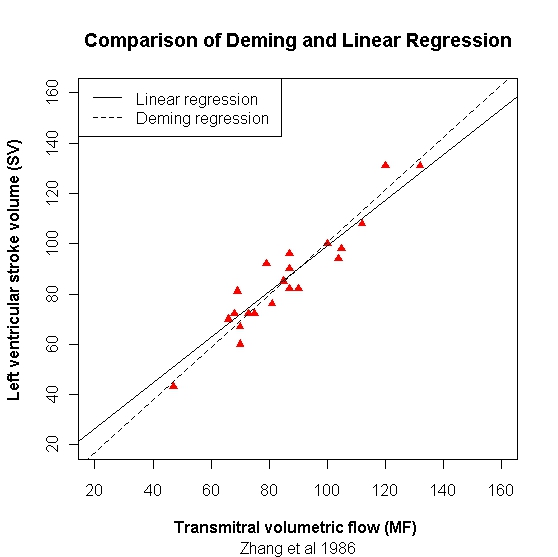
\includegraphics[width=130mm]{images/ZhangDeming.jpeg}
		\caption{Deming Regression For Zhang's Data}\label{ZhangDeming}
	\end{figure}
	
	Deming's Regression suffers from some crucial drawback. Firstly it
	is computationally complex, and it requires specific software
	packages to perform calculations.Secondly it is uninformative
	about the comparative precision of two methods of measurement.
	Most importantly \citet{CarollRupert} states that Deming's
	regression is acceptable only when the precision ratio ($\lambda$,
	in their paper as $\eta$) is correctly specified ,but in practice
	this is often not the case, with the $\lambda$ being
	underestimated.

	\subsection{Deming's Regression}
	The most commonly known Model II methodology is known as Deming's
	Regression, (also known an Ordinary Least Product regression).
	Deming regression is recommended by \citet*{CornCoch} as the
	preferred Model II regression for use in method comparison
	studies. As previously noted, the Bland Altman Plot is
	uninformative about the comparative influence of proportional bias
	and fixed bias. Deming's regression provides independent tests for
	both types of bias.
	
\bigskip
	
	As with conventional regression methodologies, Deming's regression
	calculates an estimate for both the slope and intercept for the
	fitted line, and standard errors thereof. Therefore there is
	sufficient information to carry out hypothesis tests on both
	estimates, that are informative about presence of fixed and
	proportional bias.
	

\bigskip


	


	

	\section*{Deming Regression}
	
	\begin{itemize}
		\item Informative analysis for the purposes of method comparison, Deming Regression is a regression technique taking into account uncertainty in both the independent and dependent variables.
		
		\item Deming’s method always results in one regression fit, regardless of which variable takes the place of the predictor variables.
		
		%Significant error in the least-squares slope estimation occurs when the ratio of the standard deviation of measurement of a single x value to the standard deviation of the indepedent variable data set exceeds 0.2.
		
		%Errors in the least-squares coefficients attributable to outliers can be avoided by eliminating data points whose vertical distance from the regression line exceed four times the standard error the estimate.
		
		\item The measurement error (lambda or $\lambda$) is specified with measurement error variance related as 
		\[\lambda = \sigma^2_y/\sigma^2_x\]
		
		(where $\sigma^2_x$ and $\sigma^2_y$ is the measurement error variance of the $x$ and $y$ variables, respectively).
		
		\item In the case where $\lambda$ is equal to one, (i.e. equal error variances), the methodology is equivalent to \textit{\textbf{orthogonal regression}}.
		
		\item Deming approaches the matter by simultaneously minimizing the sum of the square of the residuals of both variables. This derivation results in the best fit to minimize the sum of the squares of the perpendicular distances from the data points.
		
		\item To compute the slope by Deming’s formula,  normally distributed error of both variables  is assumed, as well as a constant level of imprecision throughout the range of measurements.
		
	\end{itemize}
	

%%%%%%%%%%%%%%%%%%%%%%%%%%%%%%%%%%%%%%%%%%%%%%%%%%%%%%%%%%%%%%%%%%%
Evaluation of Regression Procedures for Methods Comparison Studies
Kristian Linnet

%-------------------------------------------------------------------%
Comparison of Two Clinical Chemistry Methods by Regression Analysis

\[ x_i = X_i + \varepsilon_i \]
\[ y_i = Y_i + \delta_i \]

%-------------------------------------------------------------------%

% OLR
% Deming Regresssion
% Weighted Deming Regression

%-------------------------------------------------------------------%

Passing and Bablok
Performance of Regression Methods
RMSE

%-------------------------------------------------------------------%
Outliers and Non-Gaussian Error Distributions

%-------------------------------------------------------------------%
% Linnet 1998

Application of Deming Regression


Squared Analytical Error Ratio $\lambda$

Bias of the Slope Estimate

Estimation of the Deming Regression Line

\[ \beta_{OLR} =  \frac{\beta}{1 + \frac{SD^2_{ax}}{SD^2_{X}}}\]
\newpage

%%%%%%%%%%%%%%%%%%%%%%%%%%%%%%%%%%%%%%%%%%%%%%%%%%%%%%%%%%%%%%%%%%%%%%%%%%%%%%%

\subsection{Difference with Least Squares Regression}
Least-products regression can lead to inflated SEEs and estimates
that do not tend to their true values an N approaches infinity
(Draper and Smith, 1998).
	
\section*{Deming regression}
The Deming regression line is estimated by minimizing the sums of squared deviations in both the x and y directions at an angle determined by the ratio of the analytical standard deviations for the two methods.
This ratio can be estimated if multiple measurements were taken with each method, but if only one measurement was taken with each method, it can be assumed to be equal to one.
	

\section*{Deming Regression}

Performance of Deming regression analysis in case of misspecified analytical error ratio in method comparison studies

%-----------------------------------------------------------------------------------------------%
Application of Deming regression analysis to interpret method comparison data presupposes specification of the 
squared analytical error ratio ($\lambda$, but in cases involving only single measurements by each method, this 
ratio may be unknown and is often assigned a default value of one. 

On the basis of simulations, this practice was evaluated in situations with real error ratios deviating from one. 
Comparisons of two electrolyte methods and two glucose methods were simulated. 

In the first case, misspecification of $\lambda$ produced a bias that amounted to two-thirds of the maximum bias of the 
ordinary least-squares regression method. Standard errors and the results of hypothesis-testing also became misleading. 
In the second situation, a misspecified error ratio resulted only in a negligible bias. 

Thus, given a short range of values in relation to the measurement errors, it is important that $\lambda$ is correctly 
estimated either from duplicate sets of measurements or, in the case of single measurement sets, specified from 
quality-control data. However, even with a misspecified error ratio, Deming regression analysis is likely to perform 
better than least-squares regression analysis.

\newpage
\begin{verbatim}
Fiducial approach for assessing agreement between two instruments
CM Wang and Hari K Iyer
1 Statistical Engineering Division, National Institute of Standards and Technology, Boulder,
CO 80305, USA
2 Department of Statistics, Colorado State University, Fort Collins, CO 80523, USA

\end{verbatim}

%-----------------------------------------------------------------------------------------------%
%DEMING REGRESSION
This paper presents an approach for making inferences about the intercept and slope of a linear
regression model when both variables are subject to measurement errors. The approach is
based on the principle of fiducial inference. A procedure is presented for computing
uncertainty regions for the intercept and slope that can be used to assess agreement between
two instruments. Computer codes for performing these calculations, written using open-source
software, are listed.
%-----------------------------------------------------------------------------------------------%

\section*{EQUIVALENCE REGION}
The equivalence region is specified by the user. It can be an ellipse, parallelogram,
rectangle, or a region of some other appropriate shape. The way we use the fiducial region in this method is as follows. If
the $1−\gamma$ fiducial region that we construct is completely inside the equivalence region then we have established agreement.

%MAXIMUM ALLOWABLE DIFFERENCE
maximum allowable difference of the two equivalent methods.

%-----------------------------------------------------------------------------------------------%
In this paper we have provided an approach for making inference on the intercept $\beta_0$ and slope $\beta_1$ of a linear regression
model with both X and Y subject to measurement errors. Specifically, we have provided procedures for constructing
uncertainty regions for ($\beta_0$, $\beta_1$ ) that can be used to assess agreement between two methods. The approach is based on
fiducial inference.


\section*{Koning}
http://www.springerlink.com/content/r1063462u618q483/

Use of deming regression in method comparison studies.
Henk Konings

\begin{itemize}
\item Accuracy is closeness to the true value, or alternatively, having a low measurement error.

\item The determination of a true value for a biological specimen is difficult and sometimes impossible.

\item Precision is expressed in terms of standard deviation, coefficient of variance or variance.

\item In Deming regression, the errors between methods are assigned to both methods in proportion to the variances of the methods.
\end{itemize}


	\section{Linnet - References}
	The statistical procedures are described in:
	Linnet K. Necessary sample size for method comparison studies based on regression analysis. Clin Chem 1999; 45: 882-94.
	Linnet K. Performance of Deming regression analysis in case of misspecified analytical error ratio in method comparison studies. Clin Chem 1998; 44: 1024-1031.
	Linnet K. Evaluation of regression procedures for methods comparison studies. Clin Chem 1993; 39. 424-432.
	Linnet K. Estimation of the linear relationship between measurements of two methods with proportional errors. Stat Med 1990; 9: 1463-1473.
	
	
	\section{Implementation of Deming Regression with \texttt{R}s}
	Thus far, one of the few \texttt{R} implementations of Deming regression is contained in the `MethComp' package. \citep{BXC2008}.
	
	Unless specified otherwise, the variance ratio $\lambda$ has a default value of one. A means of computing likelihood functions would potentially allow for an algorithm for estimating the true variance ratio.
	
	
	
	
	%\citet{linnet93} defines analytical standard deviation as the standard deviation of measures values around the target value.\citet{linnet93} defines analytical standard deviation as the standard deviation of measures values around the target value.
	
	
\bibliographystyle{chicago}
\bibliography{DB-txfrbib}
\end{document}
	